\documentclass[11pt,a4paper]{article}
\usepackage[T1]{fontenc}
\usepackage[utf8]{inputenc}
\usepackage{lmodern}
\usepackage[margin=1in]{geometry}
\usepackage{microtype}
\usepackage{amsmath,amssymb,booktabs,tabularx,array}
\usepackage{graphicx,subcaption}
\usepackage{tikz}
\usetikzlibrary{arrows.meta,positioning,fit,calc}
\usepackage{hyperref}
\usepackage{xcolor}
\usepackage{natbib}
\usepackage{enumitem}
\hypersetup{colorlinks=true,linkcolor=blue,citecolor=blue,urlcolor=blue}
\newcommand{\LTD}{\textsc{LTD-Attack}}
\newcommand{\Hybrid}{\textsc{LTD-Hybrid}}
\newcommand{\Micro}{\textsc{LTD-Micro}}
\newcommand{\Macro}{\textsc{LTD-Macro}}
\newcommand{\futureb}{Future-B}
\newcommand{\dev}{Historical DEV}
\newcommand{\pp}{\,pp}
\title{LTD-Attack: Longitudinally Informed Website Fingerprinting under Temporal Distribution Shift}
\author{Anonymous authors\\\small Working manuscript --- non-submission version}
\date{Working draft --- 6 November 2026}
\begin{document}
\maketitle
\begin{abstract}
Website fingerprinting (WF) infers visited websites from observable patterns in encrypted Tor traffic. Although modern classifiers can recognize traffic collected under conditions resembling those of their training data, temporal changes in website content and collection environments can substantially impair generalization. We investigate whether longitudinal traffic information, used alongside a conventional within-visit fingerprint, can improve classification under temporal distribution shift. We evaluate \LTD{}, a model family comprising within-trace (micro), longitudinal (macro), and hybrid configurations, under a chronological training protocol that restricts fitting and model selection to historical development data. We report results on two previously inspected, retrospective evaluation cohorts, covering 65 websites: 09B (14,687 traces) and Future-B (18,543 traces). The hybrid attains 97.440\% and 49.453\% accuracy, respectively, compared with 95.002\% and 43.116\% for its micro-only configuration. On Future-B, it also exceeds Deep Fingerprinting (37.464\%), VarCNN (33.447\%), a CUMUL-style SVM (7.733\%), and a WFlib-based Tik-Tok implementation (20.105\%). Paired block-day analyses of the DF and VarCNN comparisons yield exploratory evidence of larger Future-B accuracy, while additional comparisons and the contrastive NetCLR baseline remain pending. Since evaluation cohorts were examined during method development, the results should not be interpreted as prospective or causally isolating concept drift. The findings motivate longitudinally informed WF as a candidate for improving performance under temporal shifts, while highlighting the need for independent prospective validation.

\end{abstract}
\noindent\textbf{Keywords:} Website fingerprinting; Tor; concept drift; longitudinal traffic analysis; encrypted traffic classification; temporal generalization.
\tableofcontents
\clearpage
\section{Introduction}\label{sec:introduction}
Tor conceals the content and destination of network communications from many local observers, but the encrypted packets that traverse a monitored link retain observable traffic characteristics. Website fingerprinting (WF) exploits such side-channel information to estimate which website a client visits. Deep Fingerprinting (DF) demonstrates that learned features can be highly discriminative in closed-world settings \citep{sirinam2018deep}; later work extends the modeling of temporal dependencies within traffic traces \citep{zhou2024transformer}.

High accuracy on temporally proximate samples does not, however, guarantee sustained performance. Changes in web content, third-party objects, browser or Tor behavior, and acquisition conditions can alter trace distributions even when the monitored websites remain nominally the same. Prior studies have emphasized the difficulty of realistic WF evaluation and the implications of evolving data distributions \citep{jansen2024repositioning,shusterman2026drift}. Models assessed only on randomly partitioned captures risk presenting an overly favorable picture of their temporal generalization.

This paper studies a complementary question: can information about repeated website observations augment the evidence contained in an individual traffic trace? The \LTD{} family contrasts a micro representation of a single website visit with a macro representation intended to encode longitudinal traffic characteristics, and examines their combination in a hybrid classifier. The aim is not to assume that every temporal change is identity-bearing. Instead, we test whether a carefully constrained complementary representation improves classification on later observations, while recognizing that predictive gains alone do not establish a causal explanation.

Our current evidence comes from a retrospectively assembled, 65-class closed-world experiment. Model selection for the new SOTA baselines is conducted solely within Historical DEV. The two external evaluation cohorts, 09B and Future-B, are held fixed at evaluation time and aligned by capture identifier, but were accessible during earlier research iterations. Consequently, all reported comparisons are explicitly retrospective. The design is intended to support reproducible and transparent interpretation rather than to imply a prospective blind test.

\paragraph{Contributions.} This working version makes four evidence-bounded contributions:
\begin{enumerate}[leftmargin=*]
\item A longitudinally informed WF research question and a micro/macro/hybrid model family evaluated under temporal distribution shift.
\item A documented chronological baseline protocol, with explicit development partitions, source provenance, frozen checkpoint selection, and aligned evaluation cohorts.
\item A comparison of \Hybrid{} with its component models and four implemented SOTA baselines (DF, VarCNN, CUMUL-style SVM, and Tik-Tok), exposing the considerable heterogeneity of temporal generalization.
\item An exploratory date-block statistical analysis for DF and VarCNN, together with an explicit account of limits from post-hoc inspection, changing collection conditions, and incomplete independent validation.
\end{enumerate}

\noindent\textbf{Completion note.} Contrastive NetCLR, the expanded paired-inference family, and a separately acquired prospective Dataset C are not represented as completed experiments here.

\section{Background and Related Work}\label{sec:related}
\paragraph{Deep website fingerprinting.} Deep Fingerprinting (DF) introduced convolutional feature learning for WF \citep{sirinam2018deep}. Temporal representations and more recent neural architectures have further broadened the range of learnable features \citep{zhou2024transformer}. Our benchmark additionally includes two WFlib implementations, VarCNN and Tik-Tok, with provenance of the specific source checkout preserved in the experimental record. Direct comparisons must account for architectural choices as well as representation and training-budget differences.

\paragraph{Temporal drift and realistic measurement.} The consequences of deployment conditions and longitudinal variation have motivated reevaluations of real-world WF performance \citep{jansen2024repositioning}. Augmentation-based robustness has been explored as an alternative to depending exclusively on a static training distribution \citep{bahramali2023realistic}; concept-drift studies have considered the consequences of evolving network traces and possible mitigation strategies \citep{shusterman2026drift}. Rather than retraining on future observations in the present frozen comparison, our protocol restricts model fitting to Historical DEV.

\paragraph{The scope of the present claim.} Longitudinal descriptors should not be conflated with additional traffic observed at inference time unless the deployment setting makes that information available. A full audit of construction and availability of macro features is required before claiming realistic online feasibility; this issue is treated as an explicit validity threat in Section~\ref{sec:validity}. The current study evaluates one fixed, 65-site, closed-world task and does not establish open-world performance.

\paragraph{Bibliography verification.} The six entries imported from the authors' preliminary ACM workshop manuscript are bibliographic starting points; title, venue, page ranges, and DOI metadata should be checked individually before submission. Full source attribution for VarCNN, CUMUL, Tik-Tok, and NetCLR will be finalized in the camera-ready bibliography after upstream-to-paper verification.

\section{Problem Setting and Threat Model}\label{sec:threat}
We consider a \emph{closed-world} WF setting in which an observer attempts to identify one of $K=65$ monitored websites from an encrypted Tor traffic trace. A trace $x_i$ contains observable packet-level information in its original capture order; each example is associated with a website label $y_i\in\{1,\ldots,K\}$, an acquisition date $d_i$, and a stable capture identifier $u_i$.

A conventional classifier models $p_\theta(y\mid x_i)$. The proposed family introduces a longitudinal context representation $z_i$ derived from traffic characteristics associated with repeated observations. Its hybrid form conceptually predicts
\begin{equation}
 \hat y_i=\arg\max_{k\in\{1,\dots,K\}} f_{\theta}(x_i,z_i)_k.
 \label{eq:hybrid}
\end{equation}
This expression is intentionally model-agnostic. Exact encoder layers, feature dimensions, normalization, fusion weights, and final score combination must be transcribed from the frozen trained implementation and verified before the architecture figure and method equations can be finalized.

\paragraph{Attacker access and assumptions.} The attacker is assumed to observe direction, timing, and other packet metadata on a monitored Tor connection, not decrypted page contents. The benchmark uses known monitored classes. Training and evaluation share the 65-class label vocabulary; unknown-site detection is outside this evaluation. The provenance and online availability of longitudinal context are part of the model assumptions, not something that can be inferred from accuracy results.

\paragraph{Temporal distribution shift.} Let $P_{\mathrm{dev}}(X,Y)$ and $P_{\mathrm{eval}}(X,Y)$ denote the joint distributions represented by historical training and later evaluation cohorts. We use \emph{temporal distribution shift} descriptively when the sampled traces differ. Accuracy degradation alone cannot determine whether the underlying mechanism is concept drift, covariate shift, acquisition artifacts, or combinations thereof. We therefore avoid causal drift attribution absent additional diagnostics.

\section{Datasets and Chronological Protocol}\label{sec:data}
\paragraph{Historical DEV.} The frozen development corpus comprises 57,916 unique captures from 65 website labels. DEV\_EARLY has 19,098 traces, DEV\_MIDDLE has 20,160, and DEV\_LATE has 18,658. Baseline phase B trains on EARLY+MIDDLE ($n=39,258$) and selects the model using DEV\_LATE; phase C refits the frozen recipe using the complete 57,916 historical traces. These data form the sole basis for fitting or selecting S7--S9 baselines.

\paragraph{Retrospective evaluation cohorts.} Cohort 09B contains 14,687 traces observed on 11 dates. Future-B (identifier 10B\_DEV\_FROZEN) contains 18,543 traces observed on 16 dates. The cohorts have 65 closed-world labels and are separately aligned by identifier, date, and class index. Results across cohorts should not be treated as paired visits of the same capture.

\begin{table}[htbp]
\centering
\caption{Observed corpus partitions and their roles. Historical DEV is the sole training/selection source for SOTA baselines. Evaluation cohorts were previously inspected and are not prospectively blinded.}
\label{tab:datasets}
\begin{tabular}{llrr}
\toprule
Partition & Role & Traces & Dates \\
\midrule
DEV\_EARLY & Baseline-B fit & 19,098 & --- \\
DEV\_MIDDLE & Baseline-B fit & 20,160 & --- \\
DEV\_LATE & Baseline-B selection & 18,658 & --- \\
Historical DEV total & Baseline-C refit & 57,916 & --- \\
09B & Retrospective evaluation & 14,687 & 11 \\
Future-B & Retrospective evaluation & 18,543 & 16 \\
\bottomrule
\end{tabular}
\end{table}


\paragraph{Frozen evaluation discipline.} Model preprocessing and selection must be established without reference to either evaluation cohort. External evaluation uses a single frozen phase-C model per baseline. All comparisons require a one-to-one UID agreement, class-order agreement, finite score arrays, and checksums of model and inference artifacts. The observed historical baseline pipelines follow this protocol, but the evaluation cohorts had been inspected during earlier stages of the broader study. We therefore distinguish \emph{frozen execution} from a \emph{prospective blind test}.

\paragraph{Temporal capture quality.} For Tik-Tok's historical timing preparation, 195,691 negative consecutive timestamp differences were detected among the 57,916 historical traces. Original frame order was preserved; no silent timestamp reordering was applied. This count measures observed backward steps and does not directly equal the number of affected captures. Device clock behavior and timestamp quality should be investigated and reported separately.

\paragraph{Prospective extension.} Dataset C is being recollected through a direct, non-bridge Tor acquisition stack and is not used in the results in this manuscript. Its eligibility as a separate test depends on acquisition and clock-quality checks, label compatibility, and a freeze of all model and decision rules preceding any analysis of that dataset.

\section{Proposed Method: LTD-Attack}\label{sec:method}
\LTD{} is organized around two complementary temporal scales. The \emph{micro} branch represents packet-level behavior within an individual page visit, whereas the \emph{macro} branch is intended to represent longitudinal characteristics across repeated observations. The hybrid combines their outputs to make a closed-world website prediction. This distinction follows the original research hypothesis, but this manuscript does not assume that the architecture described in the preliminary workshop summary is identical to the current frozen implementation.

\paragraph{Within-visit representation.} A micro encoder extracts information from individual packet sequences. Its concrete learned representation, sequence length, channel semantics, CNN/Transformer structure, and checkpoint provenance must be derived from the final implementation before submission. In particular, the earlier three-page abstract described a 3,000-packet CNN--Transformer, which is a historical description rather than verified documentation of the currently evaluated checkpoint.

\paragraph{Longitudinal representation.} The macro branch captures engineered descriptors or temporal summaries of repeated website observations. The earlier manuscript used 45 selected features and a heuristic fusion weight; neither number should be carried forward as an established property of the frozen model without a source-to-checkpoint audit. The crucial methodological questions are how a daily profile is constructed, what histories are allowed at prediction time, and whether class-conditioned aggregation could introduce information that would be unavailable to an actual observer.

\paragraph{Fusion and decision.} The currently evaluated model family includes Micro, Macro, and Hybrid variants. We deliberately use the abstract fusion notation in Eq.~\eqref{eq:hybrid} until the frozen training code, feature selection, XGBoost role, and score-combination recipe have been traced end-to-end. This is preferable to publishing a visually polished but inaccurate model diagram.

\paragraph{Diagram plan.} Figure~\ref{fig:research-pipeline} is an \emph{editable TikZ diagram of the experimental research workflow}, not yet a definitive diagram of the trained network internals. After code audit, a separate camera-ready Figure 1 will show exact encoder layers, longitudinal aggregation, fusion operations, and output head, with a common SVG source for future animation.
\begin{figure}[htbp]
\centering
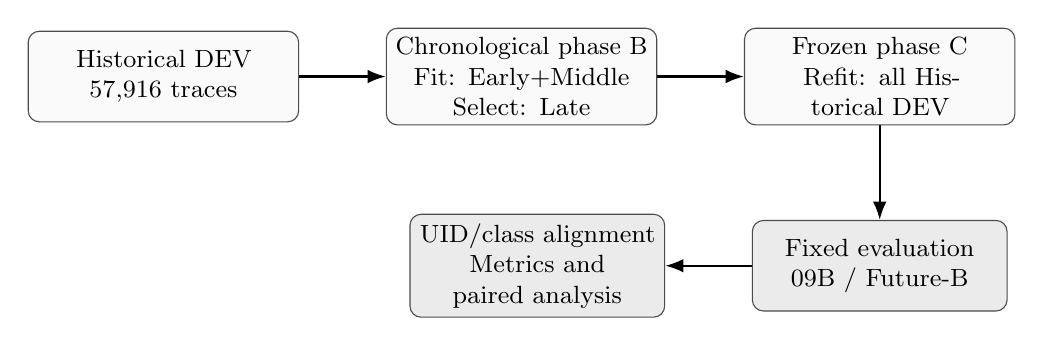
\begin{tikzpicture}[>=Latex, node distance=5mm and 11mm,
  every node/.style={font=\small},
  stage/.style={draw=black!70,rounded corners,align=center,text width=3.2cm,minimum height=1.15cm,fill=black!2},
  eval/.style={draw=black!70,rounded corners,align=center,text width=3.0cm,minimum height=1.15cm,fill=black!8}]
\node[stage] (dev) {Historical DEV\\57,916 traces};
\node[stage,right=of dev] (b) {Chronological phase B\\Fit: Early+Middle\\Select: Late};
\node[stage,right=of b] (c) {Frozen phase C\\Refit: all Historical DEV};
\node[eval,below=12mm of c] (test) {Fixed evaluation\\09B / Future-B};
\node[eval,left=of test] (audit) {UID/class alignment\\Metrics and paired analysis};
\draw[->,thick] (dev)--(b);
\draw[->,thick] (b)--(c);
\draw[->,thick] (c)--(test);
\draw[->,thick] (test)--(audit);
\end{tikzpicture}
\caption{Editable diagram of the experimental pipeline, \emph{not} the final internal neural architecture. Phase B selection and phase C refit use only historical development data; 09B and Future-B are frozen retrospective evaluations.}
\label{fig:research-pipeline}
\end{figure}


\section{Experimental Design}\label{sec:experiments}
\paragraph{Evaluated models.} We compare \Micro{}, \Macro{}, and \Hybrid{} with four implemented baselines: WFlib DF, WFlib VarCNN, a 104-dimensional CUMUL-style RBF-SVM, and WFlib-based Tik-Tok. Contrastive NetCLR is the fifth planned SOTA baseline; its outcomes are not available at the time of this manuscript version.

\paragraph{Baseline fitting.} DF and VarCNN were fitted to Historical DEV, with DEV\_LATE used for selection and phase-C refit performed after fixing the selected training length. CUMUL-style uses 104 traffic statistics and an RBF SVM with $C=1$ and scale-dependent $\gamma$. Its packet-size extraction may include protocol-header overhead and should not be called an exact reproduction of the original CUMUL method. Tik-Tok consumes directional timestamps of length 5,000 and uses the fixed WFlib architecture, Adamax at learning rate $2\times10^{-3}$, and an epoch selected on DEV\_LATE by macro-F1. Its phase-B best epoch was 23, followed by a 23-epoch phase-C refit over all Historical DEV observations.

\paragraph{Metrics.} We report top-1 accuracy, macro-averaged F1, top-5 accuracy, and mean reciprocal rank (MRR) computed from the frozen $K=65$ score vector. Macro-F1 reflects site-level imbalance; MRR reflects the position of the correct site in the complete ranking. Values are computed independently within each cohort.

\paragraph{Scope and reproducibility.} The same aligned capture identifiers and labels are required for every model in a cohort. The published values are single-run results, not claims of cross-seed stability. Hardware, environment versions, training duration, and architecture provenance should be documented for each method. NetCLR will be reported as WFlib-adapted because its practical contrastive recipe differs from the upstream batch size and dataset regimen.

\section{Results}\label{sec:results}
\begin{table}[htbp]
\centering
\small
\caption{Frozen model comparison. Accuracy, macro-F1, and top-5 are percentages; MRR is a unitless rank score. Values for LTD and DF/VarCNN come from S6; CUMUL-style from S7; Tik-Tok from S8. NetCLR not yet evaluated.}
\label{tab:main}
\setlength{\tabcolsep}{4pt}
\begin{tabular}{llrrrr}
\toprule
Cohort & Model & Acc. & Macro-F1 & Top-5 & MRR \\
\midrule
09B & LTD-Micro & 95.002 & 94.818 & 99.020 & 0.9685 \\
 & LTD-Macro & 84.068 & 83.946 & 98.523 & 0.9039 \\
 & \textbf{LTD-Hybrid} & \textbf{97.440} & \textbf{97.379} & \textbf{99.816} & \textbf{0.9853} \\
 & DF & 93.423 & 93.239 & 99.163 & 0.9593 \\
 & VarCNN & 97.290 & 97.216 & 99.775 & 0.9840 \\
 & CUMUL-style & 69.994 & 68.944 & 93.253 & 0.8023 \\
 & Tik-Tok & 94.110 & 93.858 & 99.135 & 0.9632 \\
\midrule
Future-B & LTD-Micro & 43.116 & 44.134 & 72.399 & 0.5615 \\
 & LTD-Macro & 22.305 & 18.328 & 57.995 & 0.3865 \\
 & \textbf{LTD-Hybrid} & \textbf{49.453} & \textbf{49.262} & \textbf{80.559} & \textbf{0.6306} \\
 & DF & 37.464 & 36.192 & 75.020 & 0.5358 \\
 & VarCNN & 33.447 & 31.140 & 67.244 & 0.4880 \\
 & CUMUL-style & 7.733 & 2.849 & 33.646 & 0.2265 \\
 & Tik-Tok & 20.105 & 18.557 & 52.214 & 0.3535 \\
\bottomrule
\end{tabular}
\end{table}

\paragraph{Temporally proximate evaluation (09B).} The hybrid attains 97.440\% accuracy, compared with 95.002\% for Micro and 84.068\% for Macro. The strongest SOTA comparator in this cohort is VarCNN at 97.290\%, a difference of only $0.150\pp$ from the hybrid. In the original S6 family, the hybrid--VarCNN accuracy contrast is not statistically distinguishable under the reported Holm adjustment; we therefore do not characterize the 09B result as confirmed superiority over VarCNN.

\paragraph{Later evaluation (Future-B).} All evaluated models undergo a substantial decrease in top-1 accuracy relative to 09B. The hybrid reaches 49.453\% accuracy and 49.262\% macro-F1 on Future-B, compared with Micro (43.116\%, 44.134\%), Macro (22.305\%, 18.328\%), DF (37.464\%, 36.192\%), and VarCNN (33.447\%, 31.140\%). The CUMUL-style SVM and Tik-Tok achieve 7.733\% and 20.105\% accuracy, respectively. These results are descriptive comparisons until the expanded paired-inference family is completed.

\paragraph{Temporal deterioration.} The hybrid's observed accuracy declines by 47.987 percentage points from 09B to Future-B; the corresponding differences for Micro, Macro, DF, and VarCNN are 51.886, 61.763, 55.959, and 63.843 points. The cohorts consist of different captures, so these differences characterize cross-cohort changes rather than paired changes for individual visits. This is consistent with a serious temporal generalization problem, but cannot by itself partition the effect among website evolution, software environments, and measurement conditions.

\paragraph{Incomplete comparisons.} No NetCLR accuracy, paired p-value for CUMUL/Tik-Tok, or Dataset C result is reported in this version. This omission is deliberate: the scientific narrative must not depend on anticipated findings.

\section{Paired Inference and Statistical Protocol}\label{sec:statistics}
\paragraph{Existing S6 analysis.} The frozen S6 comparison applies a paired block-by-date bootstrap with 2,500 resamples, reporting percentile 95\% intervals. A conditional paired-day label-swap procedure produces p-values, exact for accuracy, top-5, and MRR, and Monte Carlo for macro-F1, with a Holm correction across eight predeclared (within S6) contrasts per cohort (two baselines by four metrics). These inference results are retrospective and exploratory because evaluation cohorts were examined previously and consecutive day blocks may not be exchangeable.

\paragraph{09B.} For hybrid minus DF accuracy, the point difference is $4.017\pp$; the S6 reported confidence interval for the reverse comparison (DF minus Hybrid) is $[-4.596,-3.550]\pp$, with Holm-adjusted $p=0.0078125$. Hybrid minus VarCNN is $0.150\pp$; for VarCNN minus Hybrid, the interval is $[-0.384,0.088]\pp$, with Holm-adjusted $p=0.825$. The latter provides no clear evidence of a population-level advantage in 09B under the exploratory S6 procedure.

\paragraph{Future-B.} The hybrid exceeds DF and VarCNN by $11.988\pp$ and $16.006\pp$ in accuracy, respectively. The S6 intervals for DF minus Hybrid and VarCNN minus Hybrid are $[-13.090,-10.866]\pp$ and $[-17.084,-14.971]\pp$. Their reported Holm-adjusted p-values are $0.000244140625$ each. These are conditional, post-hoc results and should not be reinterpreted as prospective trial-level error guarantees.

\paragraph{Planned unified statistical analysis.} The eventual main-paper inference will incorporate the additional baselines, with UID-preserving score alignment and a prespecified family of contrasts. The existing S6 Holm-eight values will remain documented but must not be assigned to S7--S9. Dependence across consecutive dates, alternative block lengths, and additional uncertainty from one training seed require dedicated sensitivity analysis. Until then, differences involving CUMUL-style and Tik-Tok are descriptive only.

\section{Discussion}\label{sec:discussion}
Our retrospective evaluations expose a discrepancy between strong performance on 09B and substantially weaker performance on Future-B. The hybrid retains a higher fraction of top-1 accuracy than several comparator models across the two cohorts, yet even its later accuracy remains below 50\%. Robustness is therefore relative, not immunity to temporal degradation.

The difference between micro-only and hybrid performance is compatible with the hypothesis that a complementary representation helps classification. However, an apparent hybrid advantage may also depend on the fusion mechanism, an additional classifier, feature engineering, or training choices. We will isolate these factors through the existing frozen ablation evidence and, where necessary, further Historical-DEV-only experiments. Causal language about longitudinal information should be reserved for contrasts that actually hold the relevant alternatives fixed.

A second consideration concerns deployment. If macro features depend on labeled historical observations of each monitored website, the attacker must be capable of maintaining such a reference history. If the macro branch uses information from a queried visit's future or from labels unavailable at inference time, its operational interpretation would be substantially narrower. We will audit the construction window, labeling assumptions, and update rules in the code before making any deployment claim.

The CUMUL-style and Tik-Tok baselines illustrate that matching the chronological protocol does not automatically make architectures and preprocessing choices equivalent to their original publications. In particular, the CUMUL-style byte representation and the WFlib-adapted NetCLR settings require transparent deviation tables. Our goal is a fair, inspectable benchmark with appropriately qualified scope rather than an unqualified claim of state-of-the-art superiority.

\section{Threats to Validity and Research Ethics}\label{sec:validity}
\paragraph{Retrospective selection.} Future-B was previously inspected during the broader project. The 65-site class set may also be conditioned on availability of later observations. Consequently, fixed-score analysis is not equivalent to a previously unseen, prospectively held-out test, and the inference is exploratory.

\paragraph{Acquisition confounders.} Timestamp discontinuities, Tor/browser version variation, client geography, network path, crawler instrumentation, and capture scheduling may influence the measured distribution. A change in classifier performance is not, in isolation, identification of a particular drift mechanism. Capture metadata, negative timestamp steps, and source hashes will be released or summarized as permitted.

\paragraph{Representation availability.} A longitudinal profile could inadvertently exploit site-conditioned aggregates or temporal information not available at decision time. This possibility must be ruled out by tracing the final data construction and inference code. The original three-page workshop proposal is not sufficient evidence of the implemented architecture.

\paragraph{Benchmark limitations.} The present benchmark is 65-class, single-tab, closed-world Tor traffic. It does not evaluate open-world base rates, background traffic, multiclass unknown rejection, deployed defenses, user behavioral variation, or broader site families. Single-seed point estimates do not quantify variability across training runs.

\paragraph{Responsible measurement.} The uploaded workshop draft states that traces were collected by automated visits to public websites through isolated Tor clients and that no human users were monitored. These statements should be reverified against collection logs, data retention practices, and institutional ethics guidance before submission. The reported analysis concerns security evaluation and its implications for Tor users' privacy, not interception of individual people's browsing histories.

\section{Conclusion}\label{sec:conclusion}
We evaluated a longitudinally informed website-fingerprinting model family under chronological development and retrospective external testing. LTD-Hybrid achieved 97.440\% accuracy on 09B and 49.453\% on Future-B, outperforming the evaluated micro-only configuration and several conventional baselines in the later cohort. Paired day-block evidence for the DF and VarCNN contrasts supports an exploratory advantage under the analysis assumptions, but it does not constitute a prospective blind confirmation. The results suggest that combining complementary traffic representations merits further investigation, while the continued degradation of all methods highlights the difficulty of temporal generalization. Finishing the contrastive NetCLR benchmark, auditing longitudinal feature availability and ablations, and obtaining a genuinely independent later cohort are the essential next steps before advancing stronger robustness claims.

\appendix
\section{Reproducibility Checklist}\label{app:repro}
This appendix enumerates the evidence required before submission. A checkmark in the project tracking file must point to an actual immutable result, not simply an executed command.
\begin{enumerate}[leftmargin=*]
\item Immutable source code revision, WFlib upstream commit and blob checksums, and hardware/software inventory.
\item Historical DEV manifest containing UID, site-label mapping, date split, and file hashes.
\item All phase-B hyperparameters and selection metrics, plus phase-C checkpoint and training-set provenance.
\item Per-example probability artifacts for 09B and Future-B with verified UID/date/class-order alignment.
\item Complete SOTA statistics, uncertainty estimation, multiple-testing family, and cluster-date assumptions.
\item Final trained LTD micro/macro/hybrid architecture audit: inputs, transformations, fusion, XGBoost role, and online feature availability.
\item Per-model training time, resource usage, seed controls, checkpoint cadence, and run logs.
\item Prospective Dataset C integrity gate and full embargo on model/decision tuning from that cohort, if used.
\end{enumerate}
\paragraph{Evidence paths.} Recorded frozen results are preserved in the repository's
\path{docs/research/article_evidence/} directory, including the S6, S7,
and S8 result manifests dated 2026-11-06. Underlying checkpoint manifests
remain on Perseo and require independent, read-only reconciliation before release.

% Portable bibliography fallback for runtimes without BibTeX.
% references.bib remains the authoritative editable bibliographic source.
\begin{thebibliography}{9}
\bibitem[Sirinam et~al.(2018)]{sirinam2018deep}
P. Sirinam, M. Imani, M. Juarez, and M. Wright.
Deep Fingerprinting: Undermining Website Fingerprinting Defenses with Deep Learning.
\emph{ACM CCS}, 1928--1943, 2018. doi:10.1145/3243734.3243768.
\bibitem[Bahramali et~al.(2023)]{bahramali2023realistic}
A. Bahramali, A. Bozorgi, and A. Houmansadr.
Realistic Website Fingerprinting By Augmenting Network Traces.
\emph{ACM CCS}, 1035--1049, 2023. doi:10.1145/3576915.3616639.
\bibitem[Jansen et~al.(2024)]{jansen2024repositioning}
R. Jansen, R. Wails, and A. Johnson.
Repositioning Real-World Website Fingerprinting on Tor.
\emph{WPES}, 124--140, 2024. doi:10.1145/3689943.3695047.
\bibitem[Shusterman et~al.(2026)]{shusterman2026drift}
A. Shusterman, R. David, and Y. Oren.
Understanding and Addressing Concept Drift in Website Fingerprinting.
\emph{Computer Networks}, 275:111811, 2026. doi:10.1016/j.comnet.2025.111811.
\bibitem[Zhou et~al.(2024)]{zhou2024transformer}
Q. Zhou, L. Wang, H. Zhu, T. Lu, and V. S. Sheng.
WF-Transformer: Learning Temporal Features for Accurate Anonymous Traffic Identification by Using Transformer Networks.
\emph{IEEE TIFS}, 19:30--43, 2024. doi:10.1109/TIFS.2023.3318966.
\end{thebibliography}

\end{document}
